\chapter{Introduction}

\section{The Limits of the Continuous Manifold}
For over a century, General Relativity has successfully modeled the macroscopic universe by treating the vacuum as a continuous, smooth manifold. However, this assumption encounters fundamental limitations when extrapolated to the quantum limit or the Cosmic Horizon, often yielding non-physical singularities.

While the standard cosmological model ($\Lambda$--CDM) is observationally robust, it requires the introduction of phenomenological components---Dark Energy (roughly 69\%) and Dark Matter (roughly 26\%)---which dominate the cosmic energy budget yet lack a definitive micro-structural definition. Furthermore, persistent tensions in the Hubble constant ($H_0$) and the ongoing challenge of unifying gravity with quantum mechanics suggest that purely continuous, purely geometric frameworks may be operational approximations of a deeper, discrete mechanical reality. While approaches like Loop Quantum Gravity and Superfluid Vacuum Theory \cite{Rovelli_1998, Volovik_2003} have attempted to quantize space, they often remain mathematically abstract without yielding the specific macroscopic density ratios observed in astrophysics.

\section{The Spacetime Gravitational Floor (SGF)}
This paper proposes a paradigm shift from continuous geometry to discrete continuum mechanics, introducing Tension Field Theory (TFT). We postulate that the vacuum is not an empty void, but a high-stiffness, dual-phase material structure termed the Spacetime Gravitational Floor (SGF). Rather than relying on arbitrary parameter fitting, we derive the properties of this medium directly from the rigorous, classical geometry of sphere packing.

By modeling the observable vacuum as a Face--Centered Cubic (FCC) lattice, we demonstrate that the ``Dark Sector'' is simply the physical manifestation of the universe's baseline geometric architecture. Specifically, Dark Energy is reinterpreted as the volumetric packing fraction of the solid lattice phase (roughly 74\%), representing the stored elastic potential of the field. Dark Matter is reinterpreted as the visco-elastic damping of the interstitial condensate phase (roughly 26\%), representing the hydrodynamic impedance to motion through the geometric voids.

\section{Objectives of Part I}
To support this framework, we define a strict dual-scale architecture. The foundational ``Hard Floor'' is the Tension Substrate---a Simple Cubic (SC) lattice operating at the absolute limit of vacuum strain ($\ell_{\mathrm{S}} \approx 10^{-35}$ m). Emerging from this substrate at the characteristic microscopic boundary is the "Soft Floor"---a Face--Centered Cubic (FCC) lattice of resonant nodes ($r_{\mathrm{D}} \approx 10^{-26}$ m) that acts as the elastic carrier for transverse waves (light). 

\textit{*Note: $\ell_{\mathrm{S}}$ is numerically identical to the Planck Length ($\ell_{\mathrm{P}}$) but derived mechanically from the limit of vacuum strain saturation ($\alpha_{\mathrm{G}} = 1$). See \hyperref[app:substrate_units]{Appendix \ref*{app:substrate_units}}.}

In this first installment of the Tension Field Theory trilogy, we establish the exact mechanical constitution of this vacuum. We will derive the cosmic energy budget directly from the Kepler Conjecture, mechanize the origins of mass, light, and time, resolve the invisibility of the Dark Sector via acoustic impedance mismatch, and calculate the strict mechanical origins of the fundamental constants ($h$, $c_{\mathrm{E}}$, and $\mu_{\mathrm{D}}$). This structural derivation provides the necessary foundation to integrate macroscopic gravity and cosmic evolution in \hyperref[part:two]{Part II} and \hyperref[part:three]{Part III}.

\chapter{Foundational Framework}

\section{The Zeroth Law: The Foundational Tension Field}
\label{sec:zeroth_law}
We begin with the fundamental premise: a conserved and contiguous scalar tension field forms the absolute substrate of all physical reality. All observable manifestations---spacetime, mass, energy, and motion---emerge from its dynamics and return into it, conserving total energy. Its total content remains invariant across all physical transformations, from quantum fluctuations to cosmological evolution.

\section{The Mechanical Postulates}
\label{sec:2.2}
To translate this foundational law into observable physics, we define the following mechanisms that govern the mechanical architecture of the unified field:

\vspace{0.5em}
\noindent\textbf{Postulate I: The Absolute Reference Frame (The Hard Floor SC Phase)}\\
\label{postulate:one}
At the lowest limit of physical existence lies the spatially contiguous Tension Substrate---an indivisible, perfectly rigid, zero-entropy energy state, and topologically locked Simple Cubic (SC) lattice that provides the absolute reference frame for all physical mechanics.

\vspace{0.5em}
\noindent\textbf{Note:} While the discrete Substrate constitutes an absolute reference frame, Tension Field Theory recovers near-Lorentzian kinematics as an emergent Soft Floor measurement degeneracy: both the observer's apparatus and the propagating signal are covariantly deformed by the same active-vacuum mechanics (developed in \hyperref[sec:7]{Chapter 7} and Section 11.5.2). Because transverse electromagnetic propagation occurs strictly on the FCC Soft Floor rather than the Substrate, direct background sensitivity remains negligible at ordinary optical energies, leaving any extreme-energy deviations as higher-order empirical constraints.

\vspace{0.5em}
\noindent\textbf{Postulate II: Space and Time}
\label{postulate:two}
The substrate constitutes an absolute vacuum and an infinite, latent coordinate space defined by zero phase evolution ($\partial\phi/\partial t = 0$, where $\phi$ is the fundamental torsional phase angle of the lattice) and zero tension gradient ($\nabla\tau = 0$, where $\tau$ is the scalar volumetric tension). 

\begin{itemize}
    \item \textbf{Active Space} emerges strictly as the topological unfolding of substrate tension in response to phase variations.

Mechanically, Active Space is first defined by the characteristic coordinate length ($x_\phi$) generated by the discrete phase topology of the lattice nodes:
\begin{equation}
    x_\phi = \frac{\Delta\phi}{|\nabla\phi|}.
\end{equation}

The physical path length experienced by a propagating excitation is then described by the strain-weighted path functional ($D_\tau$). This functional integrates the latent coordinate path against the localized tension-gradient penalty, normalized by the absolute yield tension of the Hard Floor ($\tau_{\mathrm{S}}$) and scaled by the fundamental active-vacuum node radius ($r_{\mathrm{D}}$):
\begin{equation}
    D_\tau = \int \left( 1 + \frac{r_{\mathrm{D}}}{\tau_{\mathrm{S}}} |\nabla\tau(\mathbf{x})| \right) \mathrm{d}\ell .
\end{equation}

For a one-dimensional path from $a$ to $b$, this reduces to:
\begin{equation}
    D_\tau(a,b) = \int_a^b \left( 1 + \frac{r_{\mathrm{D}}}{\tau_{\mathrm{S}}} |\nabla\tau(x)| \right) \mathrm{d}x .
\end{equation}

   \item \textbf{Active Time} arises from the physical oscillation of the fundamental nodes within the observable space, functioning as an emergent mechanical interval that is strictly bifurcated by the topology of the field. For propagating energy (unbound waves), it functions as Coordinate Time ($t$)---the local reconfiguration interval ($\Delta t = \delta x / c_{\mathrm{P}}$, where $c_{\mathrm{P}}$ is the dynamic wave propagation speed) required for a state transfer across a locally deformed lattice region ($\delta x$). In a perfect, unstrained active space, this dynamic propagation delay minimizes to an absolute baseline constant, dictated by the fundamental coherence scale ($r_{\mathrm{D}}$) and maximum propagation potential ($c_{\mathrm{E}}$) of the lattice (defined in \hyperref[postulate:three]{Postulates III} and \hyperref[postulate:four]{IV}). Conversely, for localized mass (a bound topological defect), Active Time manifests as Proper Time ($t_{\mathrm{p}}$)---the emergent internal clock defined strictly by the accumulation of stationary, integer $360^{\circ}$ volumetric phase cycles ($n$) required to maintain localized structural equilibrium against the active vacuum.

    \vspace{0.3em}
    \textbf{Temporal Scaling Limits:}\\
    $\Delta t = \delta x / c_{\mathrm{P}}$ (where $\delta x \gg r_{\mathrm{D}}$): \textbf{Macroscopic Coordinate Time} (the lattice delay of a wave crossing a gravitational field).\\
    $\mathrm{d}t = r_{\mathrm{D}} / c_{\mathrm{E}}$: \textbf{Fundamental Coordinate Time} (the lattice delay of a wave crossing a perfect vacuum node).\\
    $t_{\mathrm{p}} = n \left( \frac{h}{E_0} \right)$: \textbf{Proper Time} (the internal clock of a localized defect, defined by its cycle count and rest energy).
\end{itemize}

\vspace{0.5em}
\noindent\textbf{Postulate III: Observable Vacuum (The Elastic Soft Floor FCC Lattice)}\\
\label{postulate:three}
The active space\index{Active Space} manifests as the observable vacuum---a contiguous Face-Centered Cubic (FCC) lattice of resonant nodes acting as the dynamic ``skin'' over the rigid substrate. This vacuum is a dual-phase visco-elastic medium composed of a solid nodal scaffold and an interstitial fluid-like condensate. The characteristic scale of these nodes is the FCC Node Radius ($r_{\mathrm{D}} \approx 10^{-26}$ m, derived in \hyperref[app:vacuum_scale_strain_unification]{Appendix~\ref*{app:vacuum_scale_strain_unification}}). This scale marks the geometric threshold where the infinite rigidity of the substrate gives way to the finite elasticity of the active vacuum, enabling dynamic phase freedom ($\Delta\phi \neq 0$), transverse oscillation, elastic deformation, and observational quantum action ($h$).

\vspace{1.0em}
\noindent\textbf{Postulate IV: The Invariant Elastic Capacity and Dynamic Propagation ($c_{\mathrm{E}}$ vs. $c_{\mathrm{P}}$)}\\
\label{postulate:four}
We differentiate the invariant elastic wave speed ($c_{\mathrm{E}}$) from the dynamic propagation velocity ($c_{\mathrm{P}}$).
\begin{itemize}
    \item \textbf{$c_{\mathrm{E}}$ (The Elastic Capacity):} Defines the field's absolute stiffness and dictates the maximum specific energy potential ($E = mc_{\mathrm{E}}^2$). This is the theoretical maximum causality limit of the active vacuum lattice ($c_{\mathrm{E}} \equiv c$).
    \item \textbf{$c_{\mathrm{P}}$ (The Dynamic Propagation):} Governs the actual transmission velocity of a propagating wave. It is determined by the local effective surface inertia ($\mu_{\mathrm{eff}}$), the baseline FCC lattice surface tension ($\tau_{\mathrm{D}}$), and the wave's phase geometry ($\Delta\phi$):
\end{itemize}
\begin{equation}
    c_{\mathrm{P}} = \sqrt{\frac{\tau_{\mathrm{D}}}{\mu_{\mathrm{eff}}}} \cdot \cos(\Delta\phi)
\end{equation}
Light represents the minimal 2D transverse shear ripple of the active vacuum, propagating through regions of baseline effective surface inertia. Mechanically:
\begin{itemize}
    \item \textbf{Hard Floor} ($\mu_{\mathrm{eff}} \to 0$): The bare substrate possesses zero intrinsic inertial density, allowing for instantaneous stress transfer ($c_{\mathrm{S}} \to \infty$).
    \item \textbf{Soft Floor} ($\mu_{\mathrm{eff}} \to \mu_{\mathrm{D}}$): In the observable vacuum, the inertia normalizes to the baseline dynamic lattice constant ($\mu_{\mathrm{D}}$), allowing the transverse wave speed to reach the invariant structural limit ($c_{\mathrm{P}} \to c_{\mathrm{E}}$).
    \item \textbf{Matter} ($\mu_{\mathrm{eff}} \gg \mu_{\mathrm{D}}$): In high-density regions (Gravity Wells), the active vacuum is subjected to macroscopic topological strain ($\alpha_{\mathrm{G}}$), which imposes two distinct mechanical impedances on the field:
    
    \vspace{0.5em}
    \textbf{Gravitational Refraction (Waves):} The amplified inertial density strictly slows the dynamic propagation speed ($c_{\mathrm{P}} < c_{\mathrm{E}}$) of transverse waves, manifesting macroscopically as the delay of Coordinate Time ($t$).
    
    \vspace{0.3em}
    \textbf{Phase Damping (Mass):} The macroscopic strain consumes a fraction of the vacuum's elastic capacity, leaving a reduced energy fraction ($1 - \alpha_{\mathrm{G}}$) available locally. This physically slows the stationary phase rotation of topological defects, expanding the duration of their emergent Proper Time ($t_{\mathrm{p}}$).
\end{itemize}

\vspace{0.5em}
\begin{samepage}
\noindent\textbf{Postulate V: Inertia, Mass, and Motion}
\label{postulate:five}
\begin{itemize}
    \item \textbf{Inertia} arises from the hydrodynamic coupling between a localized topological knot (a sustained phase-twist hosted on a fundamental $r_{\mathrm{D}}$ node) and the surrounding vacuum condensate. It expresses the field's \textit{hydrodynamic impedance} to any change in the propagation rate of this phase twist ($\Delta\phi \neq 0$) across the lattice.
    \item \textbf{Mass} is the quantitative measure of the hydrodynamic coupling, determined by the specific phase-amplitude ($r_{\mathrm{amp}}$) of the topological knot. It is an invariant structural property that dictates exactly how strongly the knot will resist a \textit{change in its rate} of geometric reconfiguration within the vacuum condensate.
    \item \textbf{Motion} originates from the field's mechanical tendency to minimize structural strain and relax toward equilibrium. For a localized knot, this proceeds through perfectly elastic Sequential Discrete Reconfiguration (State Transfer), actively steered by the potential gradient ($-\nabla\phi$) of the surrounding lattice tension.
\end{itemize}
\end{samepage}

\section{The Fundamental Definitions}
\label{sec:2.3}
From the mechanical architecture established in the postulates, we derive the fundamental identities of physical interaction:

\vspace{0.5em}
\noindent\textbf{Dimensional Nomenclature of the Tension Field:}
To formally distinguish the geometric manifestations of the Spacetime Gravitational Floor (SGF), we establish a strict dimensional hierarchy for the tension field:
\begin{itemize}
    \item \textbf{$\tau$ (Volumetric Tension / Energy Density):} The 3D internal rest energy density of the localized state, defined fundamentally as $\tau = \rho c_{\mathrm{E}}^2$. \textbf{Units:} $\mathrm{N/m^2}$ (or $\mathrm{J/m^3}$).
    \item \textbf{$\tau_{\mathrm{D}}$ (Surface Shear Tension):} The 2D structural restorative tension of the active FCC Soft Floor boundary. \textbf{Units:} $\mathrm{N/m}$ (or $\mathrm{J/m^2}$).
\end{itemize}

\vspace{0.5em}
\noindent\textbf{Definition I: Energy (Scalar Tension \& Phase Potential)}\\
\label{def:definition_one}
Energy is the fundamental measure of Volumetric Tension ($\tau$) integrated over a volume. High tension density corresponds to high energy density, whether as static potential (vacuum stress) or dynamic oscillation (wave amplitude).
\begin{equation}
    E = \tau \cdot V \equiv \hbar \cdot \frac{\partial\phi}{\partial t}
\end{equation}
Where $\partial\phi/\partial t$ is the rate of Phase Change within the FCC Soft Floor.

\vspace{0.5em}
\noindent\textbf(Note: The formal quantization of this identity, including the derivation of the local lattice Hamiltonian and the resolution of transverse kinetic and potential strain components, is formally detailed in \hyperref[app:photon_hamiltonian]{Appendix~\ref*{app:photon_hamiltonian}}.)

\vspace{0.5em}
\noindent\textbf{Definition II: Fundamental Force (The Tension \& Phase Gradient)}\\
\label{def:definition_two}
All physical interactions are manifestations of the Tension Gradient ($-\nabla\tau$) seeking to restore the FCC Soft Floor to its equilibrium phase state. Mechanically, a force is the FCC Soft Floor's resistance to Phase Twisting ($-\nabla\phi$). The observed ``Force'' is the restorative vector field generated by the Vacuum's tendency to minimize the Phase Defect and return the local topology to vacuum equilibrium:
\begin{equation}
    \mathbf{F} = -(\nabla\tau) V \equiv -(\nabla\phi) E
\end{equation}

\vspace{0.5em}
\noindent\textbf{Definition III: Matter (Resonant Node)}\\
\label{def:definition_three}
Matter is a persistent phase shift ($\Delta\phi \neq 0$) that manifests mechanically as a self-sustaining standing wave oscillation of the lattice node or a localized Topological Resonant knot within the FCC Soft Floor lattice, where it creates a structural ``soft spot'' relative to the rigid substrate.

For fundamental and virtual massive particles, mass is derived from the hydrodynamic impedance of the interstitial vacuum condensate. It is defined exactly by the product of the condensate density, the effective displacement volume, and the projection of the phase shift:
\begin{equation}
    m = \rho_{\mathrm{IC}} \cdot V_{\mathrm{eff}} \cdot \sin(\Delta\phi)
\end{equation}
Where:
\begin{itemize}
    \item $\rho_{\mathrm{IC}}$: The density of the Interstitial Vacuum Condensate, which is a volumetric projection of the FCC lattice's baseline surface inertia ($\mu_{\mathrm{D}}$).
    \item $V_{\mathrm{eff}}$: The effective displacement volume (The 3D space swept by the lattice oscillation).
    \item $\Delta\phi$: The Scalar Phase Shift (The deviation from vacuum equilibrium).
    \item $\sin(\Delta\phi)$: The Phase-Coupling Efficiency. It determines the exact proportion of the lattice vibration that manifests as measurable hydrodynamic impedance (mass). If $\Delta\phi \to 0$, the impedance vanishes ($m \to 0$). For a stable particle, the topology is fully orthogonal to the propagation axis ($\Delta\phi = 90^{\circ}$), resulting in maximum hydrodynamic impedance (Maximum Mass).
\end{itemize}

\vspace{0.5em}
\noindent\textbf{Definition IV: Charge (Lattice Chirality)}\\
\label{def:definition_four}
Electric Charge is the Topological Chirality (handedness) of the resonant node, representing a persistent stress vortex. Its polarity is defined by the direction of the lattice torsion with the discrete Chiral Integer ($\chi$):
\begin{itemize}
    \item \textbf{Positive ($\chi = +1$):} Right-Handed Torsion (Compression).
    \item \textbf{Negative ($\chi = -1$):} Left-Handed Torsion (Rarefaction).
    \item \textbf{Neutral ($\chi = 0$):} Zero Torsion (Symmetric Oscillation).
\end{itemize}

\vspace{0.5em}
\noindent \textbf{Definition V: Information (The Topological Strain Record)}\\
\label{def:definition_five}
Information is the permanent, mechanical ledger of the universe. It is defined as a discrete topological footprint: the specific, static longitudinal strain configuration encoded within the ultra-dense Simple Cubic (SC) Substrate (The Hard Floor).

Mechanically, as Energy (Definition I) dynamically propagates across the active FCC Soft Floor, it exerts a localized downward mechanical stress upon the substrate, registering as a discrete longitudinal strain defect.

For any dynamic state---whether a propagating wave (Photon) or a localized resonant knot (Matter)---the total information content $N$ is fundamentally defined as the ratio of the Carrier's total dynamic energy ($E_{\mathrm{carrier}}$) to the static strain energy of a single continuous record ($E_{\mathrm{record}}$).

\begin{itemize}
    \item \textbf{The Kinematic (Wave) Identity:}
    \begin{equation}
        N_{\gamma} = \frac{1}{2\pi} \left(\frac{\lambda}{\ell_{\mathrm{S}}}\right)^2
    \end{equation}
    
    \item \textbf{The Inertial (Matter) Identity:}
    \begin{equation}
        N_{\mathrm{m}} = 2\pi\left(\frac{m_{\mathrm{S}}}{m}\right)^2
    \end{equation}
\end{itemize}

Where:
\begin{itemize}
    \item $N_{\gamma}, N_{\mathrm{m}}$: The total count of discrete longitudinal strain bits (formally derived in \hyperref[app:graviton]{Appendix \ref*{app:graviton}}) anchoring the dynamic Soft Floor state to the static Hard Floor Substrate.
    \item $\lambda, m$: The macroscopic wavelength and localized inertial mass of the Soft Floor carrier.
    \item $\ell_{\mathrm{S}}, m_{\mathrm{S}}$: The fundamental Lattice Spacing and Mass Potential of the Substrate (See \hyperref[app:substrate_units]{Appendix \ref*{app:substrate_units}}).
\end{itemize}

\chapter{The Dual-Scale Architecture of the Vacuum}

\section{The Coherence Boundary and the Kinematic Ceiling}
\label{sec:coherence_boundary}
As established in \hyperref[postulate:three]{Postulate III}, the active Spacetime Gravitational Floor (SGF) is a visco-elastic medium with a finite structural capacity. To resolve the singularity paradoxes inherent in continuous field theories, Tension Field Theory (TFT) postulates an absolute microscopic Coherence Boundary. This boundary is defined by the characteristic radius of the fundamental Face-Centered Cubic (FCC) lattice node ($r_{\mathrm{D}}$), representing the smallest scale at which a transverse excitation can be coherently sustained before localized lattice saturation occurs.

\subsection{Multi-Parameter Global Calibration of the FCC Node ($r_{\mathrm{D}}$)}
The active Spacetime Gravitational Floor cannot be dimensionlessly derived; its geometric scale ($r_{\mathrm{D}}$) must be globally calibrated against the physical extremes of the observable universe. The framework must simultaneously satisfy two empirical Standard Model boundaries:

\begin{itemize}
    \item \textbf{The Low-Energy Anchor (Resting State):} The structural capacity of the vacuum must physically accommodate the $246.22$ GeV Vacuum Expectation Value (VEV) without localized fracture.
    \item \textbf{The High-Energy Consistency Check:} The physical Nyquist limit of the calibrated geometry should yield a wave-fracture scale compatible with the broad electroweak vacuum-instability range ($1.0 \times 10^{10}$ to $1.0 \times 10^{12}$ GeV).
\end{itemize}

The fundamental node radius is calibrated by equating the mass-equivalent electroweak VEV scale to the physical hydrodynamic capacity of the Interstitial Condensate ($\rho_{\mathrm{IC}}$), defined in \hyperref[app:fcc_constants]{Appendix~\ref*{app:fcc_constants}}, occupying the total Interstitial Volume ($V_{\mathrm{IC}}$), detailed in \hyperref[sec:lattice_packing]{Section~\ref*{sec:lattice_packing}}, of a single Face-Centered Cubic cell ($\approx 25.95\%$ of the cell volume). By defining the 3D vacuum fluid density from the linear gravitational mass-density scale of the lattice ($c_{\mathrm{E}}^2/G$), projected volumetrically through the macroscopic SI calibration convention ($\iota_{\mathrm{V}} \equiv 1~\mathrm{m}^{-1}$), we formulate a calibrated geometric matching condition.

The complete step-by-step calibration calculation is provided in \hyperref[app:vacuum_scale_strain_unification]{Appendix~\ref*{app:vacuum_scale_strain_unification}}. This calibration should not be read as a parameter-free derivation of $r_{\mathrm{D}}$ from the Standard Model; rather, it establishes the empirical active-vacuum scale used throughout the TFT framework. Solving the calibrated matching condition yields:
\begin{equation}
r_{\mathrm{D}} \approx 7.4504 \times 10^{-27}~\mathrm{m}.
\end{equation}

In subsequent sections, this fundamental dimension $r_{\mathrm{D}}$ governs the mechanical manifestations of the active vacuum. (Note: Because the coefficient $7.45$ falls above the logarithmic midpoint of a base-10 scale ($\sqrt{10} \approx 3.16$), the fundamental geometric grain size is strictly classified as an order-of-magnitude scale of $r_{\mathrm{D}} \sim 10^{-26}$ m in all subsequent expressions of the FCC node size).

\subsection{Post-Calibration Consistency Check Against the Kinematic Ceiling \texorpdfstring{($E_{\mathrm{max}}$)}{E\_max}}
To confirm this geometric calibration is physically valid, the calibrated node radius is evaluated against the absolute Kinematic Ceiling ($E_{\mathrm{max}}$). Because a transverse wave knot cannot physically propagate through a lattice node smaller than its own physical diameter ($\lambda_{\mathrm{min}} = 2r_{\mathrm{D}}$), this limit represents the absolute energy required to compress a singular photon's spatial wavelength to the physical diameter of the node, triggering structural lattice failure.

Utilizing the internal kinematic equation for a localized photon-like excitation ($E = hc_{\mathrm{E}}/\lambda$), the fracture limit of the calibrated SGF evaluates to:
\begin{equation}
    E_{\mathrm{max}} = \frac{hc_{\mathrm{E}}}{2r_{\mathrm{D}}}
\end{equation}

Using the invariant constant $hc_{\mathrm{E}} \approx 1.2398 \times 10^{-15} \text{ GeV}\cdot\text{m}$:
\begin{equation}
    E_{\mathrm{max}} = \frac{1.2398 \times 10^{-15} \text{ GeV}\cdot\text{m}}{2(7.4504 \times 10^{-27} \text{ m})} \approx 8.3203 \times 10^{10} \text{ GeV}
\end{equation}

The resulting value lies within the broad electroweak vacuum-instability range often quoted in Standard Model extrapolations. Because $r_{\mathrm{D}}$ has already been empirically calibrated using the electroweak VEV scale, this agreement should be interpreted as a post-calibration consistency check rather than as an independent prediction. The result shows that the calibrated FCC Soft Floor scale is not immediately incompatible with the expected high-energy structural instability window.

\vspace{0.5em}
\noindent\textbf{Composite vs. Fundamental Saturation:}\\
It is critical to distinguish this geometric ceiling from the observed energies of Ultra-High-Energy Cosmic Rays (UHECRs) \cite{Bird_1995, PierreAuger_2014}. A UHECR is a macroscopic composite structure (a proton) that distributes its immense kinetic energy across millions of resonant nodes via a hydrodynamic shockwave. The limit $E_{\mathrm{max}}$ defines the absolute Nyquist yield threshold strictly for a \textit{single, fundamental transverse wave} (such as a single photon).

\section{The Scale Hierarchy and the Cosmic Boundary}
\label{sec:scale_hierarchy}
While the microscopic boundary ($2r_{\mathrm{D}}$) is calibrated to the empirical limits of the Standard Model, the macroscopic boundary of the universe is governed by the structural dissipation of the active vacuum. Tension Field Theory utilizes these two absolute limits to define the total scale hierarchy of the local cosmic domain.

\subsection{The Kinematic Boundary ($R_{\mathrm{U}}$)}
Because the active Spacetime Gravitational Floor is a visco-elastic medium, transverse shear waves cannot propagate infinitely. Their kinetic energy is continuously subjected to a fundamental, macroscopic temporal Vacuum Damping Rate ($\Gamma_{\mathrm{D}}$).

Observational cosmology measures this visco-elastic damping directly as the Hubble parameter ($H_0 \equiv \Gamma_{\mathrm{D}}$). Using the SH0ES collaboration baseline of $H_0 \approx 73.0$ km/s/Mpc, the absolute kinematic limit of macroscopic wave coherence is calculated. Standard cosmology identifies this distance as the Cosmic Horizon. In Tension Field Theory, this boundary is mechanically defined as the Viscous Cosmic Horizon.

The Viscous Cosmic Horizon ($R_{\mathrm{U}}$) is the characteristic coordinate distance at which the visco-elastic damping of the lattice attenuates a propagating wave by a factor of $1/e$ (draining approximately $63.2\%$ of its initial kinematic energy):
\begin{equation}
    R_{\mathrm{U}} = \frac{c_{\mathrm{E}}}{\Gamma_{\mathrm{D}}} = \frac{c_{\mathrm{E}}}{H_0} \approx 1.2665 \times 10^{26} \text{ m}
\end{equation}

\subsection{The Kinematic Lattice Index ($N_{\mathrm{D}}$)}
The macroscopic limit of coherence ($R_{\mathrm{U}}$) and the microscopic limit of coherence ($2r_{\mathrm{D}}$) establish the absolute mechanical phase boundaries of the active vacuum. These bounds are synthesized into a single, fundamental dimensionless invariant: the Kinematic Lattice Index ($N_{\mathrm{D}}$).
\begin{equation}
    N_{\mathrm{D}} = \frac{R_{\mathrm{U}}}{2r_{\mathrm{D}}} = \frac{1.2665 \times 10^{26} \text{ m}}{2(7.4504 \times 10^{-27} \text{ m})} \approx 8.4995 \times 10^{51}
\end{equation}

\vspace{0.5em}
\noindent\textbf{Physical Meaning:}\\
$N_{\mathrm{D}}$ represents the characteristic maximum number of discrete lattice nodes a transverse excitation can traverse before visco-elastic damping reduces its kinematic energy below the $1/e$ macroscopic coherence threshold. Because $N_{\mathrm{D}}$ is a pure dimensionless ratio bounded by fundamental geometry and empirical observation, it is an absolute structural property of the visco-elastic continuum.

\subsection{The Quantum-Cosmic Consistency Identity}
\label{sec:quantum_cosmic_identity}
This dimensionless scale ratio mathematically bridges the microscopic and macroscopic boundaries of the universe. Rather than treating these limits as isolated phenomenological parameters, Tension Field Theory demonstrates they form a strict Scale-Invariant Identity. Projecting the macroscopic temporal damping ($\Gamma_{\mathrm{D}}$) across the total geometric lattice count ($N_{\mathrm{D}}$) yields the exact mathematical equivalence of the quantum vacuum's energetic yield limit:
\begin{equation}
    E_{\mathrm{max}} \equiv h \Gamma_{\mathrm{D}} N_{\mathrm{D}}
\end{equation}

Rather than an independent derivation, this identity serves as a rigorous structural consistency check. It demonstrates that the scale kinematics of the FCC vacuum commute perfectly across extremes: the localized ultraviolet structural cutoff ($E_{\mathrm{max}}$) is strictly equivalent to the infrared cosmic decay rate ($\Gamma_{\mathrm{D}}$) integrated across the absolute spatial depth of the lattice. (The formal proof of this strain unification is detailed in \hyperref[app:vacuum_scale_strain_unification]{Appendix~\ref*{app:vacuum_scale_strain_unification}}).

\begin{figure}[H]
\centering
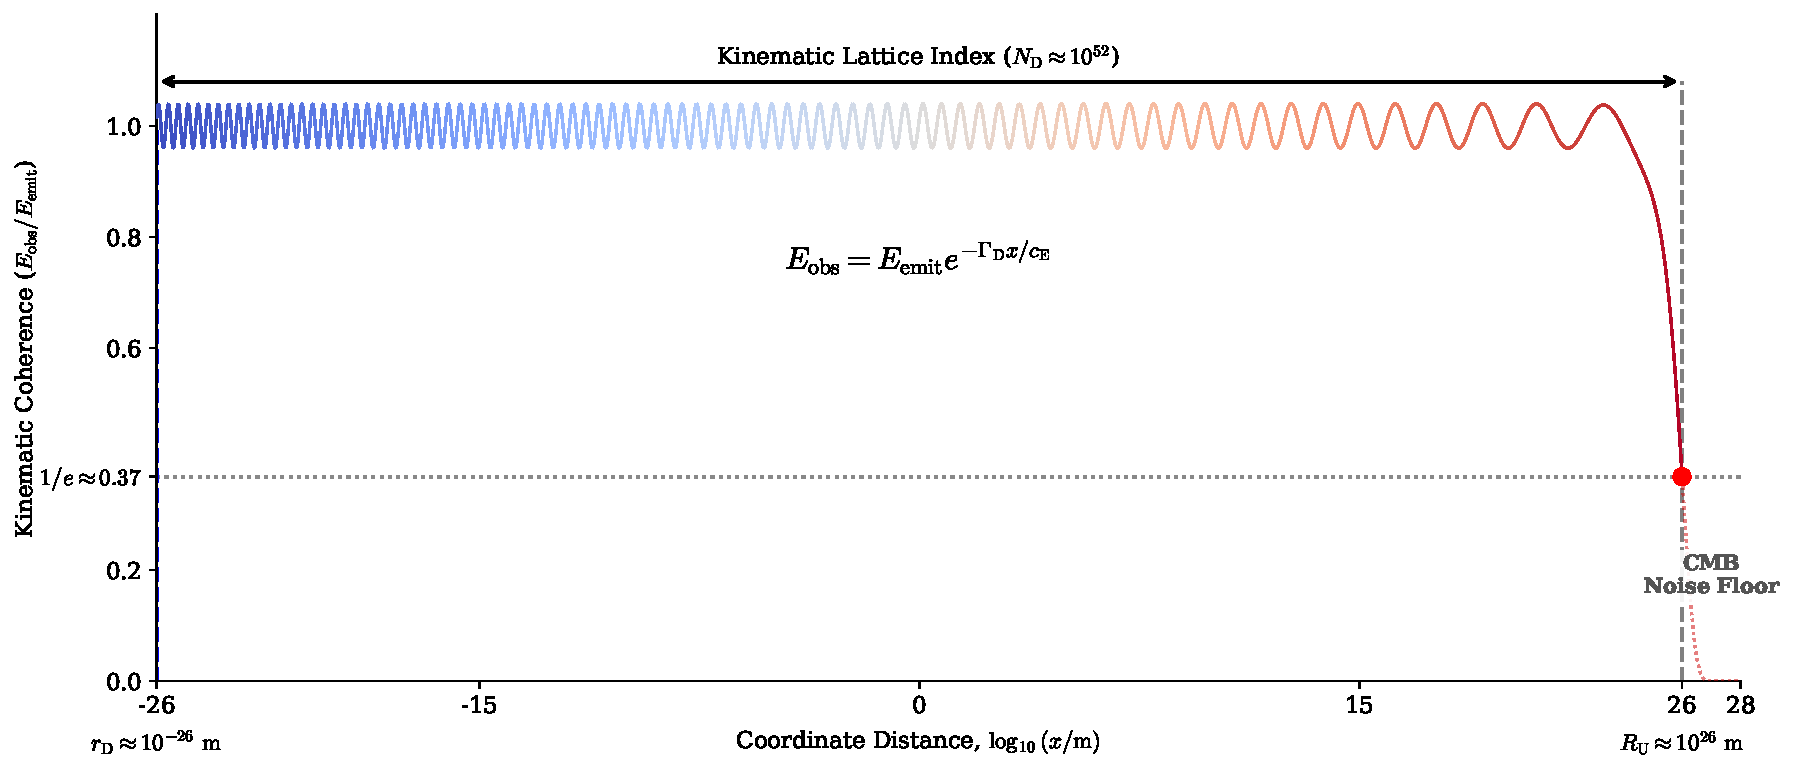
\includegraphics[width=0.9\textwidth]{Fig01_PartI_ViscousCosmicHorizon.pdf}
\caption{\textbf{The Scale Hierarchy of the Active Vacuum.} The observable universe exists within a finite structural envelope spanning approximately 52 orders of magnitude ($N_{\mathrm{D}} \approx 10^{52}$). It is bounded on the micro-scale by the lattice resolution limit ($r_{\mathrm{D}} \approx 10^{-26}$ m), where quantum saturation triggers a phase transition, and on the macro-scale by the Viscous Cosmic Horizon ($R_{\mathrm{U}} \approx 10^{26}$ m), where lattice damping ($\Gamma_{\mathrm{D}}$) exponentially attenuates the wave's kinematic energy by a factor of $1/e \approx 0.37$.
\newline \textbf{Wave Kinematics:} The visual represents a propagating transverse wave undergoing continuous visco-elastic damping. The vertical amplitude strictly follows the exponential decay equation ($E_{\mathrm{obs}}$), while topological conservation of the wave packet causes the horizontal wavelength to continuously elongate, generating the cosmological redshift ($1+z$). Beyond $R_{\mathrm{U}}$, the wave sheds its remaining energy into the ambient $2.725$ K Cosmic Microwave Background \cite{Fixsen_2009} (thermal exhaust).}
\label{fig:scale_hierarchy_boundary}
\end{figure}

\section{The Constitution of the SC Phase Hard Floor Substrate}
As established in \hyperref[postulate:one]{Postulate I}, the Latent Substrate acts as the absolute mechanical foundation of the universe. Operating at the terminal boundary of physical compression, its mechanical properties are defined by strict mathematical limits:
\begin{itemize}
    \item \textbf{The Irreducible Node Spacing:} This is the Substrate Lattice Spacing ($\ell_{\mathrm{S}}$)---the terminal structural boundary where geometric compression halts and gravitational saturation is absolute. It is defined by the vacuum yield limit: $F_{\mathrm{S}} = c_{\mathrm{E}}^4/G$.
    \item \textbf{Latent State Energy:} In this absolute vacuum state, the substrate possesses maximal latent structural energy ($E_{\mathrm{S}} = c_{\mathrm{E}}^4 \ell_{\mathrm{S}}/G$) but strictly zero intrinsic inertial density ($\mu_{\mathrm{S}} \to 0$).
    \item \textbf{Longitudinal Transmission:} The absolute structural stiffness of the unit cell ($F_{\mathrm{S}}/\ell_{\mathrm{S}}^2$) combined with its zero intrinsic inertia allows for instantaneous stress transfer through longitudinal transmission without the localized transfer of energy.
\end{itemize}

\begin{figure}[H]
    \centering
    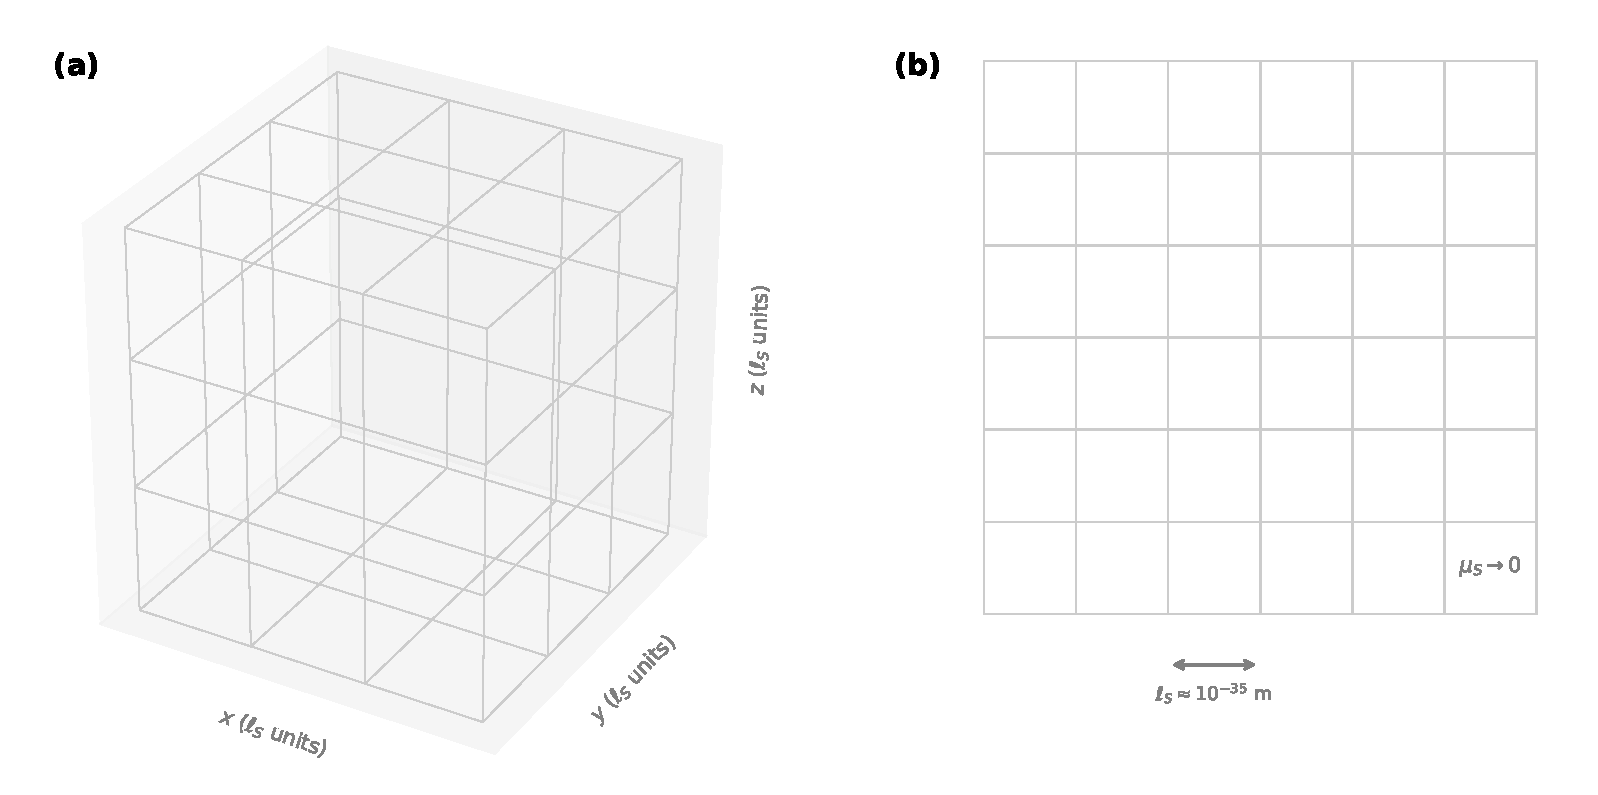
\includegraphics[width=0.8\textwidth]{Fig02_PartI_Substrate.pdf}
  \caption{\textbf{The Latent Substrate ($\tau = \tau_{\mathrm{S}}$).} The fundamental vacuum architecture is a rigid Simple Cubic (SC) lattice at the structural limit $\ell_{\mathrm{S}} \approx 10^{-35}$ m. \textbf{(a) The Volumetric Core (Equilibrium Phase):} A 3D illustration of the topologically locked phase ($\phi_{\mathrm{S}} = 0$). This visualizes the field's maximum rigidity ($F_{\mathrm{S}} = c_{\mathrm{E}}^4/G$), which maintains the structural integrity of the absolute vacuum in its equilibrium state. \textbf{(b) The Lattice Projection (Reference Frame):} A 2D depiction of the absolute reference frame---an incompressible grid ($K_{\mathrm{S}} \to \infty$) with zero intrinsic effective inertia ($\mu_{\mathrm{S}} \to 0$) that strictly defines the coordinate system for the maximal tension field.}
\label{fig:substrate}
\end{figure}

\subsection{The Three Topological States of the Field}
While this foundational substrate is an invariant continuum, the field operates in three distinct topological states relative to its equilibrium:
\begin{itemize}
    \item \textbf{State 0: The Latent Substrate (Equilibrium, $\tau = \tau_{\mathrm{S}}$):} The invisible ``Hard Floor'' of reality. The lattice remains in its fundamental SC configuration with zero intrinsic inertial density ($\mu_{\mathrm{S}} \to 0$), providing instantaneous mechanical connectivity ($c_{\mathrm{S}} \to \infty$) of the universe.
    \item \textbf{State I: The Active Vacuum (Expansion, $\tau = \tau_{\mathrm{D}}$):} The dynamic ``FCC Soft Floor'' (Spacetime). Acting as an elastic skin over the rigid substrate, the nodes reconfigure into a Face--Centered Cubic (FCC) geometry, enabling transverse waves (Light) and interstitial inertia (Mass).
    \item \textbf{State II: The Saturated Core (Compression, $\alpha_{\mathrm{G}} \to 1$):} The ``Frozen Phase'' (Black Holes). When gravitational saturation occurs, the active FCC skin undergoes a structural phase transition to the underlying internally phase-locked Substrate floor, eliminating interstitial voids and mechanically arresting time.
\end{itemize}

\begin{table}[H]
\centering
\caption{Summary of the SC Phase Substrate Constants (See \hyperref[app:substrate_units]{Appendix \ref*{app:substrate_units}} for the mechanical definitions of these values)}
\label{tab:substrate_constants}
\renewcommand{\arraystretch}{1.4}
\begin{tabular}{@{}ll l p{6.5cm}@{}}
\toprule
\textbf{Property} & \textbf{Symbol} & \textbf{Mathematical Relation} & \textbf{Mechanical Definition} \\
\midrule
Phase State & $\phi$ & $0$ & Absolute Vacuum Equilibrium \\
Coherence & $\Psi_{\mathrm{S}}$ & $\sqrt{n_0} \cdot e^{i0} \quad (n_0 = \ell_{\mathrm{S}}^{-3})$ & Single Macroscopic Wave Function \\
Lattice Spacing & $\ell_{\mathrm{S}}$ & $\sqrt{\hbar G / c_{\mathrm{E}}^3}$ & The 1D Spacing of the SC Lattice \\
Structural Mass Moment & $J_{\mathrm{S}}$ & $\rho_{\mathrm{S}} \ell_{\mathrm{S}}^4$ & Source of $\hbar$ and $G$ \\
Bond Force & $F_{\mathrm{S}}$ & $c_{\mathrm{E}}^4 / G$ & Maximal Lattice Yield Strength \\
Max Tension & $\tau_{\mathrm{S}}$ & $F_{\mathrm{S}} / \ell_{\mathrm{S}}^2$ & The Absolute Stress Limit \\
Latent Energy & $E_{\mathrm{S}}$ & $F_{\mathrm{S}} \cdot \ell_{\mathrm{S}}$ & Latent structural energy per cell \\
Stiffness & $K_{\mathrm{S}}$ & $\to \infty$ & Topologically Locked Phase \\
Wave Mode & --- & \text{Longitudinal Only} & Stress Update (No Energy Transfer) \\
Inertia & $\mu_{\mathrm{S}}$ & $\to 0$ & Massless Transmission Medium \\
Entropy & $S_{\mathrm{S}}$ & $0$ & Perfect Geometric Order \\
Speed & $c_{\mathrm{S}}$ & $\to \infty$ & Instantaneous State Correlation (Entanglement) \\
Absolute Substrate Index & $N_{\mathrm{S}}$ & $R_{\mathrm{Res}} / \ell_{\mathrm{S}}$ & Total dimensionless radial nodes ($\approx 3.827 \times 10^{69}$). Derived in \hyperref[sec:unified_phase_summary]{the Unified Phase Map Summary}. \\
\bottomrule
\end{tabular}
\end{table}

\subsection{The Master Geometric Scaling Law}
To transition from State 0 (The Latent Substrate) to State I (The Active Vacuum), the universe cannot simply fracture across scales; it must strictly conserve its fundamental mechanical action.

As introduced in the Substrate Constants table (\hyperref[tab:substrate_constants]{Section \ref*{tab:substrate_constants}}) and rigorously derived in \hyperref[app:conservation_action]{Appendix \ref*{app:conservation_action}}, the absolute Scale-Invariant Mass Moment of the vacuum is strictly defined as $J_{\mathrm{S}} = \rho_{\mathrm{S}} \ell_{\mathrm{S}}^4$. This invariant represents the irreducible, intrinsic structural mass moment of the field---the absolute mechanical capacity for Quantum Action ($\hbar$) prior to the emergence of kinematic mass. Because the vacuum is a contiguous elastic medium, this fundamental action must be conserved across all topological bounds.

To conserve this mechanical action while maintaining a constant transverse wave speed ($c_{\mathrm{E}}$), the localized density of the vacuum ($\rho$) must geometrically dilute as a strict function of the inverse-fourth power of the radius ($r$). This geometric projection is governed by the Master Geometric Scaling Law:
\begin{equation}
    \rho(r) = \mathcal{F}_i \cdot \rho_{\mathrm{S}} \left(\frac{\ell_{\mathrm{S}}}{r}\right)^4
\end{equation}

\noindent\textbf{Where:}
\begin{itemize}
    \item $\rho_{\mathrm{S}}$: The absolute Substrate Density ($\approx 5.1550 \times 10^{96}$ kg/m$^3$).
    \item $\ell_{\mathrm{S}}$: The 1D Substrate Lattice Spacing ($\approx 1.6162 \times 10^{-35}$ m).
    \item $r$: The radial topological scale of the localized node.
    \item $\mathcal{F}_i$: The Topological Form Factor, which accounts for the specific volumetric geometry of the localized phase state ($\mathcal{F}_{\mathrm{D}} = 1.5$ for the spherical nodes of the active Soft Floor).
\end{itemize}

\textit{(See \hyperref[app:conservation_action]{Appendix \ref*{app:conservation_action}} for the strict mathematical derivation of this scaling law, the geometric proof of the Form Factor, and the Topological Boundary Equation).}

This equation acts as the universal gear ratio of Tension Field Theory. It proves that the emergent density of the observable cosmos is not an arbitrary parameter, but a strict, deterministic projection of the underlying Hard Floor.

When this scaling law is evaluated at the FCC Node Radius ($r = r_{\mathrm{D}} \approx 10^{-26}$ m), it dictates the exact mechanical density of the observable Spacetime Gravitational Floor, setting the stage for the active vacuum.

\section{The Constitution of the FCC Phase Soft Floor Active Vacuum}
\label{sec:fcc_lattice}
While the Substrate (the Hard Floor) provides the absolute boundary conditions, the observable cosmos exists exclusively on the active Spacetime Gravitational Floor (SGF). As established in \hyperref[postulate:three]{Postulate III}, Tension Field Theory (TFT) models this Soft Floor not as a smooth, continuous geometry, but as a dual-phase visco-elastic Face--Centered Cubic (FCC) medium emerging from the substrate via symmetry breaking at the FCC Node Radius ($r_{\mathrm{D}} \approx 10^{-26}$ m).

At this scale, the active SGF acquires finite stiffness, inertia, and viscous impedance. The FCC geometry is not chosen heuristically; it is the unique close-packed spherical architecture that maximizes local connectivity while preserving interstitial freedom.

This architecture dictates that the vacuum is strictly partitioned into two inseparable, constitutive phases:
\begin{itemize}
    \item \textbf{The Solid Lattice Phase (74\% Volumetric Capacity)}
    \begin{itemize}
        \item \textbf{Geometry:} Approximately 74\% of the spatial volume is occupied by the solid, spherical FCC nodes acting as a rigid scaffold.
        \item \textbf{Constitutive Role:} This phase provides the lattice shear stiffness, surface tension, and transverse-wave support required for the propagation of light and all coherent elastic communication.
    \end{itemize}
    \item \textbf{The Interstitial Condensate Phase (26\% Volumetric Capacity)}
    \begin{itemize}
        \item \textbf{Geometry:} The remaining 26\% of the volume consists of the contiguous, interconnected void network between the FCC nodes, filled entirely by the fluid-like interstitial condensate.
        \item \textbf{Constitutive Role:} This phase provides the viscous and inertial response of the vacuum. It supplies the hydrodynamic impedance and inductive reactance associated with mass, vacuum damping, and dissipative coupling.
    \end{itemize}
\end{itemize}

\noindent\textbf{The Mechanical Stage}\\
The Soft Floor is neither a pure crystal nor a pure fluid; it is a universal, dual-phase visco-elastic medium exhibiting supersolid-superfluid mechanics. The solid lattice nodes and the interstitial condensate strictly divide the labor of reality. This exact geometric partition dictates the origins of light, mass, gravity, and dark-sector phenomena. The specific mechanical derivations of these interactions---including localized kinematic transport, impedance mismatch, and structural saturation thresholds---are systematically developed in the subsequent sections of this framework.

\begin{figure}[H]
    \centering
    \includegraphics[width=0.8\textwidth]{Fig03_PartI_FCCLattice.pdf}
    \caption{\textbf{The Active Vacuum Phase (Soft Floor FCC Architecture).} The observable vacuum manifests as a Face--Centered Cubic (FCC) structure precisely at the FCC Node Radius ($r_{\mathrm{D}} \approx 7.45 \times 10^{-27}$ m). This maximum-density packing arrangement geometrically partitions the vacuum into two distinct phases: The \textbf{Solid Nodal Scaffold} ($\rho_{\mathrm{D}} \approx 1.71 \times 10^{62} \text{ kg/m}^3$) represents the operational, vibrational density of the lattice, acting as the fundamental source of quantum action. The structural integrity of this scaffold generates the absolute lattice shear stiffness ($\tau_{\mathrm{D}}$), which provides the restorative tension for gravity and transverse wave propagation. The \textbf{Interstitial Condensate} ($\rho_{\mathrm{IC}} \approx 1.81 \times 10^{53} \text{ kg/m}^3$) is the volumetric projection of baseline inertia ($\mu_{\mathrm{D}}$), providing the fluidic response responsible for absolute hydrodynamic impedance. Together, they establish the dual-phase visco-elastic foundation of the Soft Floor.}
\label{fig:fcc_lattice}
\end{figure}

\newpage
\begin{table}[H]
\centering
\caption{Summary of FCC Phase Active Vacuum Constants (See \hyperref[app:fcc_constants]{Appendix \ref*{app:fcc_constants}} and \hyperref[app:phase_transition]{Appendix \ref*{app:phase_transition}} for the mathematical derivations of these values)}
\label{tab:soft_floor_constants}
\renewcommand{\arraystretch}{1.0} 
\begin{tabular}{@{}ll l >{\raggedright\arraybackslash}p{5.2cm}@{}}
\toprule
\textbf{Property} & \textbf{Symbol} & \textbf{Mathematical Relation} & \textbf{Mechanical Definition} \\
\midrule
Phase State & $\phi(t)$ & $\phi \neq 0$ & Dynamic Phase (Time Flow) \\
Geometry & --- & \text{FCC} & Maximum Density Packing \\
FCC Node Radius & $r_{\mathrm{D}}$ & $h c_{\mathrm{E}} / 2E_{\mathrm{D}}$ & Fundamental geometric resolution limit of the SGF \\
Kinematic Lattice Index & $N_{\mathrm{D}}$ & $R_{\mathrm{U}} / 2r_{\mathrm{D}}$ & Total dimensionless radial nodes ($\approx 8.508 \times 10^{51}$) \\
Structural Mass Moment & $J_{\mathrm{D}}$ & $\rho_{\mathrm{D}} r_{\mathrm{D}}^4$ & Lattice Structural Mass Moment (Governs observable $h$ and $G$) \\
Bulk Modulus & $\tau_{\mathrm{D,bulk}}$ & $c_{\mathrm{E}}^4 / (G \cdot r_{\mathrm{D}}^2)$ & Lattice Yield Strength \\
Shear Stiffness & $\tau_{\mathrm{D}}$ & $c_{\mathrm{E}}^4 / (G \cdot r_{\mathrm{D}})$ & Lattice Surface Tension (Source of light speed) \\
Baseline Inertia & $\mu_{\mathrm{D}}$ & $c_{\mathrm{E}}^2 / (G \cdot r_{\mathrm{D}})$ & Emergent Inertial Density for FCC lattice \\
Impedance Accel. & $a_{\mathrm{D}}^*$ & $c_{\mathrm{E}}^2 / R_{\mathrm{U}} = c_{\mathrm{E}} \cdot \Gamma_{\mathrm{D}}$ & Acceleration equivalent of vacuum impedance \\
Damping Rate & $\Gamma_{\mathrm{D}}$ & $c_{\mathrm{E}} / R_{\mathrm{U}}$ & Vacuum Damping Rate (Cosmological Redshift Mechanism) \\
Wave Speed Limit & $c_{\mathrm{E}}$ & $\sqrt{\tau_{\mathrm{D}} / \mu_{\mathrm{D}}}$ & Absolute Transverse Velocity Limit \\
Condensate & $\rho_{\mathrm{IC}}$ & $\mu_{\mathrm{D}} \cdot \iota_{\mathrm{V}}$ & Interstitial Condensate Density (Holographic Impedance) \\
Quantum Mass & $M_{\mathrm{D,Q}}$ & $\rho_{\mathrm{D}} \cdot r_{\mathrm{D}}^3$ & 3D localized inertia of a single quantum node \\
Fundamental Impedance & $K_{\mathrm{D}}$ & $\rho_{\mathrm{IC}} \cdot (4\pi r_{\mathrm{D}}^2)$ & Absolute Hydrodynamic Coupling Constant \\
Operational Node Density & $\rho_{\mathrm{D}}$ & $1.5 \cdot \rho_{\mathrm{Q}}$ & Baseline mechanical mass-density of the active FCC node \\
Gravitational Yield Density & $\rho_{\mathrm{D,G}}$ & $c_{\mathrm{E}}^2 / (G \cdot r_{\mathrm{D}}^2)$ & Structural yield density limit (Lattice bond fracture) \\
Quantum Energy Limit & $E_{\mathrm{D,Q}}$ & $h c_{\mathrm{E}} / 2r_{\mathrm{D}}$ & Kinematic saturation limit (Phase transition trigger) \\
Grav. Energy Limit & $E_{\mathrm{D,G}}$ & $\mu_{\mathrm{D}} \cdot c_{\mathrm{E}}^2 \cdot r_{\mathrm{D}}^2$ & Structural yield limit (Lattice bond fracture) \\
Node Saturation Mass & $M_{\mathrm{D,G}}$ & $c_{\mathrm{E}}^2 \cdot r_{\mathrm{D}} / G$ & Micro-Black Hole Limit (Minimum mass to structurally lock a node) \\
\bottomrule
\end{tabular}

\vspace{0.3em}
\parbox{\textwidth}{\small \textbf{Note:} The mechanical resistance of the vacuum manifests as the Lattice Impedance Acceleration ($a_{\mathrm{D}} = c_{\mathrm{E}} \cdot \Gamma_{\mathrm{D}}$), derived in \hyperref[app:cosmic_impedance]{Appendix \ref*{app:cosmic_impedance}}. This acts as the physical, structural origin of the empirical MOND constant ($a_0$), explaining the ``Dark Matter'' effect as a kinematic reality of vacuum impedance rather than an invisible particle. Here, $\Gamma_{\mathrm{D}}$ is the Vacuum Lattice Damping Rate, derived in \hyperref[app:vacuumdamping_cosmicredshift]{Appendix \ref*{app:vacuumdamping_cosmicredshift}}.}
\end{table}

\chapter{Lattice Constraints and Quantization}
The discrete architecture of the SGF imposes strict mechanical limits on physical action. ``Quantum Mechanics'' is defined here as the stress-strain constitutive law of the vacuum lattice.

\section{The Resolution Limit}
The FCC Node Radius ($r_{\mathrm{D}}$) constitutes the physical resolution limit of the vacuum.
\begin{itemize}
    \item \textbf{Constraint:} Position is physically undefined below the lattice spacing ($x < r_{\mathrm{D}}$).
    \item \textbf{Mechanism:} Attempting to localize energy below this scale induces lattice shear rather than coordinate precision, converting positional information into vibrational noise (Uncertainty).
\end{itemize}

\section{Quantization of Action (Origin of $h$)}
Energy is quantized because the Soft Floor lattice functions as a stiff resonator that physically rejects non-resonant vibrational modes.

\begin{itemize}
    \item \textbf{Mechanism:} The contiguous lattice only accepts energy transfer in discrete, whole-cycle packets sufficient to activate the full harmonic rotation of a node. Fractional phase cycles cannot propagate through the elastic medium.
    \item \textbf{Definition:} The Planck constant ($h$) is therefore not an arbitrary limit of observation, but the specific mechanical \textit{Action of Existence}---the rotational momentum required to complete one volumetric cycle of a single Soft Floor node.
\end{itemize}

As formally derived in \hyperref[app:conservation_action]{Appendix \ref*{app:conservation_action}} and \hyperref[app:fractal_architecture]{Appendix \ref*{app:fractal_architecture}}, this action is the strict kinematic product of the node's internal torsional resistance ($J_{\mathrm{D}}$) operating at the absolute elastic capacity of the field, which mechanically dictates its transverse speed limit ($c_{\mathrm{E}}$):
\begin{equation}
    h = 2\pi \cdot J_{\mathrm{D}} \cdot c_{\mathrm{E}}
\end{equation}
yielding the observable quantum of action $h \approx 6.6261 \times 10^{-34}$ J$\cdot$s.

\begin{figure}[H]
    \centering
    % Ensure Fig04_PartI_QuantumAction.pdf is placed in your "Figures" folder
    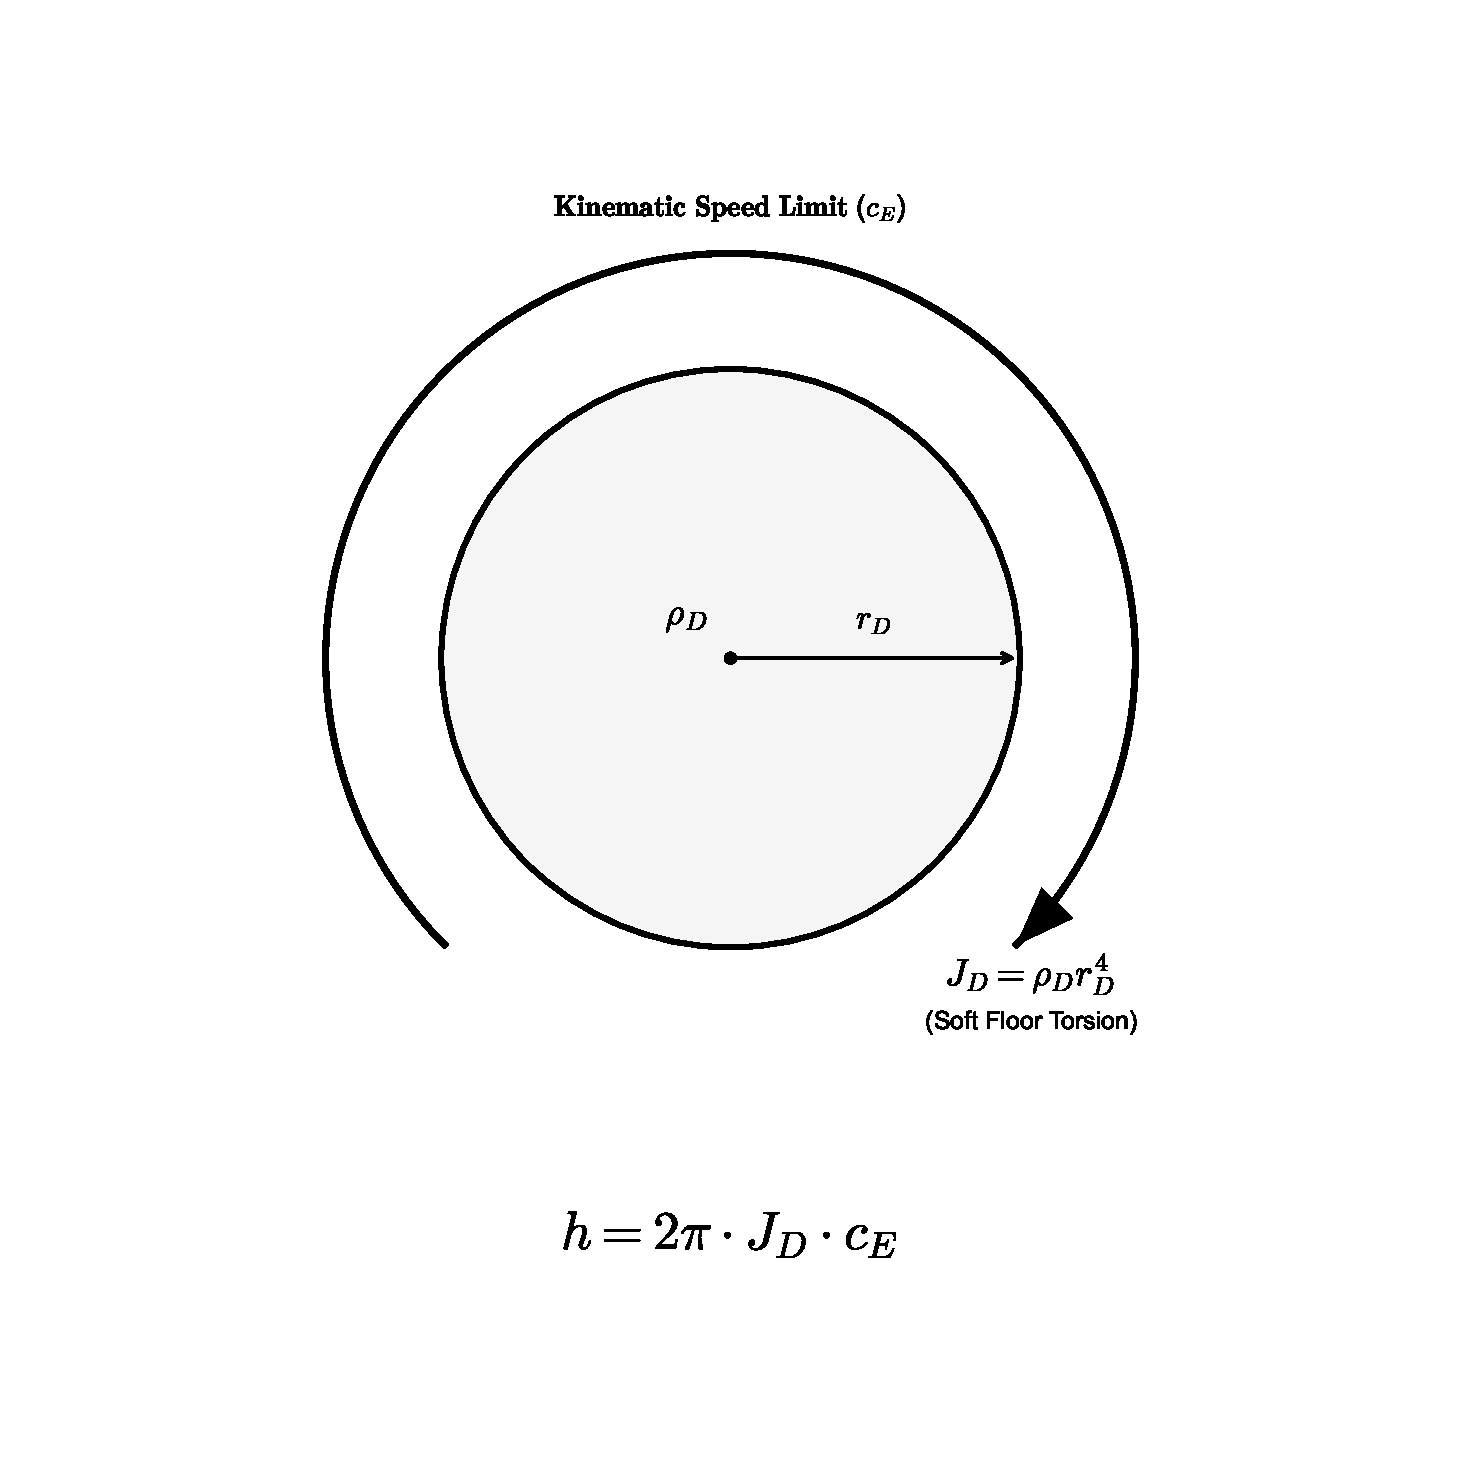
\includegraphics[width=0.85\textwidth]{Fig04_PartI_QuantumAction.pdf}
  \caption{\textbf{The Mechanical Kinematics of the Quantum of Action ($h$).} This schematic illustrates the internal rotational architecture of the localized Soft Floor node. The fundamental action ($h$) operates as an entirely self-contained kinematic property of the medium. It is defined mathematically as the direct product of the node's intrinsic Structural Mass Moment ($J_{\mathrm{D}}$), driven by the transverse kinematic speed limit ($c_{\mathrm{E}}$), and governed by the $2\pi$ geometry of the rotational phase state.}
\label{fig:quantum_action}
\end{figure}

\vspace{0.3em}
\noindent \textbf{The Geometric Requirement of Integer Cycles ($S = n h$)}

To maintain structural stability, the contiguous Face--Centered Cubic (FCC) lattice cannot sustain partial geometric phase rotations. A localized topological defect must complete a full $360^{\circ}$ volumetric rotation ($2\pi$ radians) to successfully return the surrounding vacuum nodes to their neutral, relaxed baseline; a partial cycle leaves the lattice permanently deformed under unsustainable elastic strain. 

This establishes a strict boundary condition on the accumulated macroscopic action ($S$) of any mechanical event within the medium. If the continuous phase angle of the rotation is $\phi$, the total action is defined as $S = \hbar \phi$. Because the physical lattice requires complete rotations, the phase angle must strictly equal integer multiples of $2\pi$ ($\phi = n \cdot 2\pi$, where $n = 1, 2, 3, \ldots$). Substituting this geometric requirement yields:
\begin{equation}
    S = \hbar (n \cdot 2\pi) = n h
\end{equation}

In standard quantum mechanics, $S = n h$ represents the abstract Bohr-Sommerfeld quantization postulate. In Tension Field Theory, it is the mandatory solid-state condition for structural equilibrium. Energy and action are strictly quantized because topological defects must complete full, integer rotations ($n$) to preserve the macroscopic geometric harmony of the crystal lattice.
\vspace{0.3em}

\subsection*{The Physical Translation of the De Broglie Wave}
This internal quantization directly generates the macroscopic momentum vector. In standard quantum mechanics, the instantaneous phase of a propagating plane wave is defined as $\phi(\mathbf{x},t) = \mathbf{k} \cdot \mathbf{x} - \omega t$, where the spatial gradient of the phase yields the wave vector ($\nabla\phi = \mathbf{k}$).

TFT physicalizes this relationship. Because the central node must rotate in discrete, quantized cycles ($h$) against the lattice resistance, it induces a discrete spatial phase gradient ($\nabla\phi$) in the surrounding medium. Therefore, the standard quantum momentum relation (the De Broglie equation) is not a probabilistic abstraction, but a strict continuum mechanics identity defining the physical push of the phase gradient:
\begin{equation}
    \mathbf{p} = \hbar \mathbf{k} \quad \equiv \quad \mathbf{p} = \hbar (\nabla\phi)
\end{equation}
Momentum is the mechanical projection of the node's internal action ($\hbar$) propagating across the spatial phase gradient ($\nabla\phi$) of the contiguous vacuum.

\section{The Mechanical Origin of the Pilot Wave}
The lattice architecture mechanically resolves the Wave-Particle paradox by separating the Topological Node from the Elastic Response of the Field.
\begin{itemize}
    \item \textbf{Mechanism:} The Resonant Node (Particle) generates elastic shear waves in the surrounding Soft Floor.
    \item \textbf{Result:} These waves reflect off the lattice geometry, creating a local pressure gradient that steers the node's trajectory. The particle is guided by the hydrodynamic wake of its own vibration, which is elaborated upon in \hyperref[part:two]{Part II} (\hyperref[sec:pilot_wave]{Section \ref*{sec:pilot_wave}}).
\end{itemize}